% !TeX root = ../Trabajo_RPM.tex
\section{Evaluación sobre cien instancias sintéticas}\label{sec:instancias}
En esta fase se extiende la experimentación llevada a cabo en la sección~\ref{sec:resultados} con el caso diario. Se ejecuta la regla de asignación de RPM y el MILP en cien instancias con diferentes demandas, tamaños, horizontes, capacidades y matrices de tiempos. Cada instancia es resuelta con la heurística corporativa y el solucionador CBC, HiGHS y Gurobi. Esta etapa se ilustra en la figura~\ref{fig:ruta_metodologica_rpm}, y se encuentra ubicada después de la caracterización de los datos y antes de la interpretación de planes. Mientras que los experimentos con repeticiones llevan a cabo el mismo problema, el experimento con 100 problemas consiste en observar el efecto de utilizar diferentes instancias de entrada.

\subsection{Muestra y generación de demanda}\label{sec:muestreo100}
El libro de RPM ofrece volúmenes de demanda semestrales, agrupados por referencia, pero no una serie temporal de pedidos individuales. Así, permite estudiar la heterogeneidad entre referencias, pero no permite estimar una distribución de demanda diaria para una referencia dada, ni tampoco una estacionalidad de dicha demanda. Por eso se utilizará un remuestreo estratificado transversal, y se hará explícito el supuesto necesario para utilizarlo: dentro de un volumen de demanda similar, los factores relativos de unas referencias pueden ser utilizados como donantes para construir nuevas demandas sintéticas. Esta hipótesis no es una propiedad demostrada de las ventas a través del tiempo: es el supuesto en el que se basa el experimento.

Las doscientas referencias se ordenan según sus ventas en el semestre. En caso de empate, el programa utilizado ordena por nombre, y luego divide el conjunto de referencias en tres grupos con tamaños parecidos. De esta forma se evita que la dispersión relativa de las referencias menos vendidas se mezcle directamente con la de las referencias con mayor volumen de ventas. Al mismo tiempo, se evita que alguno de los estratos quede con un número de donantes pequeño para el remuestreo con reemplazo. La tabla~\ref{tab:estratos100} muestra la dispersión de las demandas que servirá de base para el generador sintético. El coeficiente de variación del estrato de las referencias de mayor volumen de ventas es mucho mayor, y se conserva esta asimetría en el experimento en vez de aplicar a todas las referencias una perturbación aleatoria uniforme.

\begin{table}[H]\centering\small
\caption{Estratos de volumen semestral utilizados como base del remuestreo}\label{tab:estratos100}
\begin{tabular}{lrrrr}\toprule
Estrato & Referencias & Media (unidades) & Mediana & CV\\\midrule
Bajo & 67 & 3.596 & 3.439 & 0,20\\
Medio & 67 & 9.715 & 10.012 & 0,30\\
Alto & 66 & 85.758 & 32.246 & 1,60\\\bottomrule
\end{tabular}
\fuente{ventas semestrales del anexo de datos; estadísticos redondeados de \texttt{distribucion\_estratos.csv}}
\end{table}

Siendo $V_i$ la venta semestral de la referencia $i$ y $g(i)$ el estrato al que pertenece, se calcula, para cada donante $k$ del mismo grupo, el cociente $w_k=V_k/\overline V_{g(i)}$. El promedio de estos cocientes coincide con el valor 1 dentro de cada estrato. Para cada bloque $b$ se selecciona con reemplazo un donante $k(i,b)$ de ese mismo grupo que $i$ y se define la demanda del bloque $b$
\begin{equation}
	D_{ib}=\left\lfloor d_i^{\mathrm{base}}\,H_b\,\lambda_b\,\frac{V_{k(i,b)}}{\overline V_{g(i)}}+\frac12\right\rfloor,
	\label{eq:demanda100}
\end{equation}
donde $d_i^{\mathrm{base}}$ es la demanda diaria calibrada (véase el anexo \ref{an:construccion}) y $H_b$ y $\lambda_b$ son el horizonte y nivel de demanda del bloque $b$. Se ha considerado la parte entera más próxima al valor, para asegurar que la demanda sea una variable entera. Antes de aplicar esta transformación, el factor aleatorio mantiene sin alteración la demanda base en valor esperado. No ocurre lo mismo para una realización, en concreto. Los niveles de intensidad de demanda son condiciones bajo las que se experimenta, no estimas de su frecuencia en el funcionamiento real.

El diseño experimental tiene 4 niveles de intensidad de demanda (0,8; 1,0; 1,2 y 1,4), 3 tamaños de catálogo (99, 150 y 200 referencias) y 3 horizontes (1, 3 y 5 días). El número de combinaciones posibles es 36. De ellas, se ha elegido un subconjunto de 25 celdas siguiendo una regla de permutación y exclusión modular que se definió previamente al resolver los problemas. Con ella, se seleccionan 24 celdas y una adicional a éstas, elegida entre las omitidas según la semilla utilizada. Así, los niveles de demanda han sido empleados en 24, 24, 24 y 28 problemas respectivamente; los tamaños de catálogo, en 32, 32 y 36 problemas; y los horizontes, en 32, 32 y 36 problemas. Con esta fracción de diseño se incluye la experiencia de todos los niveles, pero no todos los efectos e interacciones posibles del factorial completo.

Una común modificación al catálogo del problema es hacer que existan subconjuntos anidados dentro del catálogo: los 99 productos están contenidos en los 150, los cuales están contenidos en los 200. Esto nos da una forma de manejar parcialmente como varía la composición del catálogo a medida que aumentamos su tamaño. No obstante, no consideramos todas las mezclas posibles del catálogo para igual cantidad de productos.

Cada celda de este cuadro genera un vector de demanda que se conserva en cuatro versiones: capacidad nominal o reducida en 25\,\% en M1, y matriz de demanda como fue publicada o reconstruida. La capacidad nominal es de 1.440 minutos por máquina por día, mientras que en M1 se reduce a 1.080 en la versión de capacidad reducida. Los alistamientos se mantienen en sus valores originales. De esta manera, obtenemos un total de 100 problemas distintos a partir de 25 realizaciones de demanda, sin eliminar o cambiar problemas en base a su dificultad o a si son o no factibles. La semilla utilizada para generar la demanda es 191007. En el anexo~\ref{an:instancias100} se encuentran identificadas las cien instancias y sus huellas; en el manifiesto digital se guarda la huella SHA-256 completa.

Los diferentes tamaños permiten hacer una conexión con el caso diario de 99 productos y el catálogo ampliado con 200 productos, siendo el catálogo de 150 productos un nivel intermedio. Un día permite replicar el horizonte corto, mientras que tres días permite conectarnos con el caso nominal de multiperiodo con lote, y 5 días hace que el modelo tenga que considerar un horizonte más largo. El uso de la matriz publicada y la reconstruida permite analizar la sensibilidad a los coeficientes como se hace en la sección~\ref{sec:datos}. La capacidad reducida de M1 es un ejemplo de ensayo de capacidad, y no representa una situación de parada observada en planta. Esta diferencia de datos permite no sólo analizar cómo se comparan los métodos, sino también donde una asignación conjunta supera a la regla local.

\subsection{Comparación emparejada y alcance estadístico}
La heurística implementa en forma algorítmica la regla de asignación de RPM explicada en la sección~\ref{sec:heuristica}. La extensión de esta heurística al caso multiperiodo consiste en repetir la asignación un día a la vez, ordenar la demanda insatisfecha y asignarla utilizando primero las máquinas con menor tiempo unitario disponible. La implementación de la heurística establece la forma en la que se resuelven los desempates. Todos los métodos se ejecutan sobre el mismo problema, recibiendo la misma demanda, capacidad y matriz. Como resultado, la comparación realizada no es entre diferentes heurísticas o métodos de la compañía sino que se estudia la regla utilizada por la compañía bajo diferentes entradas, controladas y conocidas. Los planes encontrados por los métodos sintéticos no deben ser tomados como los turnos que la empresa realizó en determinado momento de su historia.

Los tres motores utilizados para resolver el modelo completo del problema, presentado en la sección~\ref{sec:modelo}, tienen el mismo set de refuerzos válidos, y no se le proporciona a ninguno de los motores una solución inicial. Para verificar la correcta implementación de los motores se realizó una auditoría para chequear que el LP de cada instancia resuelto por cada motor tiene el mismo hash. Se corrió cada método una vez por cada instancia para evitar confundir la repetición de una semilla con una variedad de problemas. Se siguió un protocolo de ejecución para asignar un presupuesto de resolución a cada problema según su tamaño y horizonte. A cada problema se le asignó el mismo presupuesto de tiempo a cada uno de los motores (CBC, HiGHS, y Gurobi). Todos los motores corrieron sobre el mismo modelo con el mismo criterio de aceptación de soluciones. El detalle de este protocolo se detalla en el Anexo~\ref{an:protocolo100}. Esto significa que un problema más grande obtiene más tiempo de cómputo, en proporción a su tamaño, que uno más pequeño. Esto se hace para no favorecer a ninguno de los motores al momento de hacer la comparación. El orden de corrida de los motores se alternó entre las instancias, y debido a las diferentes condiciones de entorno donde se corrían los experimentos, las comparaciones de tiempos de resolución son más limitadas.

Si la heurística y motor resuelven el problema satisfaciendo toda la demanda, la reducción de carga es
\begin{equation}
R_{bs}=100\,\frac{Z_b^{\mathrm{heur}}-Z_{bs}}{Z_b^{\mathrm{heur}}}.
\label{eq:mejora100}
\end{equation}
Un plan parcial no es una referencia equivalente. Si en cualquiera de los dos métodos no hay demanda, el informe no hará el cálculo de la reducción, manteniendo el faltante. Tampoco el hecho que el incumbente sea mejor que la heurística lo convierte en óptimo.

Las cuatro instancias de una celda de problema tienen la demanda en común. Es decir, no son cuatro extracciones independientes. La celda comparable es la unidad sobre la que se aplica el bootstrap, manteniendo juntas las distintas variantes. Se realizaron 1.000 remuestreos con semilla 19042 en cada motor y se obtuvieron los percentiles 2,5\,\% y 97,5\,\% sobre las medias \cite{davison1997}. En el diseño hay 25 celdas, de las cuales Gurobi y HiGHS tienen 18 celdas con parejas completas, mientras que CBC tiene 16. Así, el intervalo indica el rango de variación de los resultados de las comparaciones en el diseño. El hecho que se seleccionen instancias con distintos tamaños y horizontes tampoco aísla de por sí un efecto causal, ya que las celdas tienen otras diferencias en condiciones.

\subsection{Resultados: cobertura y calidad de las soluciones}
Los cien problemas generaron los 400 registros que nos esperábamos. Las 24 instancias que los tres motores consideraron inviables fueron las mismas; a las 76 restantes se les pudo ofrecer un plan completo verificado por HiGHS y Gurobi. CBC terminó 54. La heurística consiguió encontrar una solución para 68 de las instancias y quedaron 8 de ellas con demanda insatisfecha que, sin embargo, pudo ser cubierta por el MILP. En la tabla~\ref{tab:solvers100} hemos diferenciado entre la capacidad de un plan factible y el cierre de las cotas.

\begin{table}[H]\centering\footnotesize\setlength{\tabcolsep}{5pt}
\caption{Cobertura y GAP final de la comparación central}\label{tab:solvers100}
\begin{tabular}{lrrrr}\toprule
Método & Planes completos & Óptimos acreditados & GAP mediano (\%) & GAP máximo (\%)\\\midrule
Heurística & 68 & -- & -- & --\\
CBC & 54 & 20 & 1,5423 & 13,3623\\
HiGHS & 76 & 31 & 0,6324 & 3,6061\\
Gurobi & 76 & 41 & 0,0100 & 0,1795\\\bottomrule
\end{tabular}
\fuente{consolidado de 400 registros. El GAP mediano y el GAP máximo se afectan únicamente por los planes completos sin certificado: 34 de CBC, 45 de HiGHS y 35 de Gurobi. Las 24 inviabilidades concordantes no conforman esas medianas}
\end{table}

Con Gurobi, los 76 planes completos alcanzan un GAP menor que 0,18\,\%; 68 planes tienen un GAP no mayor a 0,1\,\%. Lo cual implica que la brecha relativa entre el valor objetivo obtenido y una cota inferior válida es pequeña. El resultado de los 5 días se mantiene similar: en dicho periodo se tienen 32 planes completos, de los cuales nueve tienen un óptimo acreditado, y un GAP máximo de 0,179452\,\%. Para el caso de E097 con 200 referencias y 5 días se tiene que $LB=49.591,9587946$ y $UB=49.591,9587963$ minutos, lo cual representa un GAP de apenas $3,43\times10^{-9}\,\%$. Con el criterio de verificación, se acreditan 41 óptimos, y los otros 35 planes completos tienen cotas cercanas, representando asignaciones factibles.

\subsection{Comparación con la regla de RPM y perfil de factores}
En la tabla \ref{tab:mejora100} únicamente aplicamos la ecuación~\eqref{eq:mejora100} si ambos planes sirven a un mismo pedido. Para las 68 parejas de soluciones completas proporcionadas por Gurobi, el MILP proporciona una mejora media del 21,8\,\% sobre la carga nominal, con un intervalo de confianza bootstrap del 19,5\,\% al 24,8\,\%. Todas las 68 mejoras son positivas. Para el subconjunto de problemas para los que los tres motores fueron capaces de encontrar soluciones (48 problemas), las medias de mejora son del 21,4\,\% para CBC, del 23,1\,\% para HiGHS y del 23,2\,\% para Gurobi. Esta comparación mantiene fijo el conjunto de problemas.

\begin{table}[H]\centering\small
\caption{Reducción de carga frente a la heurística de RPM en parejas completas}\label{tab:mejora100}
\begin{tabular}{lrrrr}\toprule
Motor & Parejas & Media (\%) & Mediana (\%) & IC 95\,\% (\%) \\
\midrule
CBC & 48 & 21,4 & 20,6 & [17,9; 24,9] \\
HiGHS & 68 & 21,4 & 20,2 & [18,9; 24,5] \\
Gurobi & 68 & 21,8 & 20,3 & [19,5; 24,8] \\
\bottomrule\end{tabular}

\fuente{\texttt{comparacion\_heuristica\_100.csv}. El intervalo remuestrea las celdas comparables, no cada variante por separado; el número de parejas difiere entre motores}
\end{table}

La figura~\ref{fig:perfil100} recupera la comparación por factores de tiempo: para cada instancia con algún óptimo acreditado, divide el tiempo de cierre de cada motor por el menor tiempo acreditado de esa misma instancia \cite{dolan2002}. El factor 1 identifica al primero; un método sin cierre conserva factor infinito. El perfil mantiene como denominador los 76 problemas con plan completo. Gurobi alcanzó el primer cierre en 41 de las 42 instancias donde algún motor acreditó el óptimo; HiGHS lo hizo en la restante. Los tiempos también dependen del hardware de los trabajadores remotos. El perfil caracteriza este protocolo de ejecución y no constituye una clasificación universal de velocidad.

\begin{figure}[H]\centering
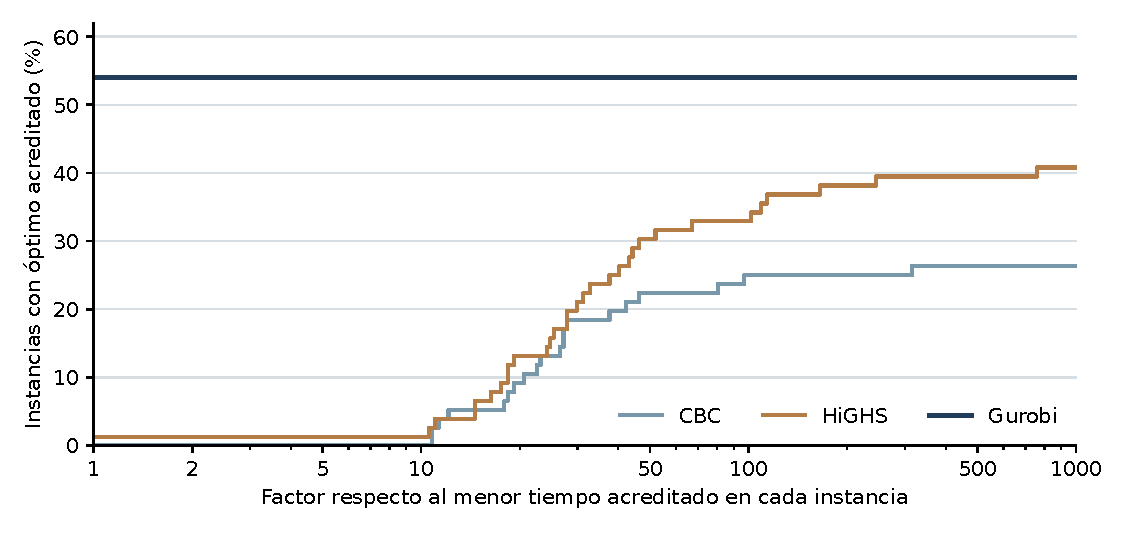
\includegraphics[width=.90\linewidth]{figuras/perfil_factores_100.pdf}
\caption{Proporción de las 76 instancias con solución factible para las que cada motor acredita el óptimo dentro del factor de tiempo indicado. Los casos sin certificado no alcanzan un factor finito.}\label{fig:perfil100}
\fuente{\texttt{consolidado\_400.csv}; cálculo reproducible en \texttt{generar\_resultados\_estratificados.py}}
\end{figure}

En la instancia nominal diaria, el modelo MILP reduce la carga agregada de producción un 15,6\,\% frente a la heurística de referencia. Por su parte, el Monte Carlo histórico tiene un valor promedio cerca del 15,2\,\% bajo la misma perturbación de demanda. Para este estudio se usaron 100 problemas en los que se modifica el tamaño, el horizonte, la matriz y la capacidad. Estas corridas no se agregan a la media. La ventaja en carga obtenida es para planes similares bajo los supuestos del modelo. En el anexo~\ref{an:instancias100} es posible localizar el estado y el GAP de cada instancia.
